\begin{figure}[ht]
	\centering
	\begin{subfigure}[ht]{\linewidth}
		\centering
		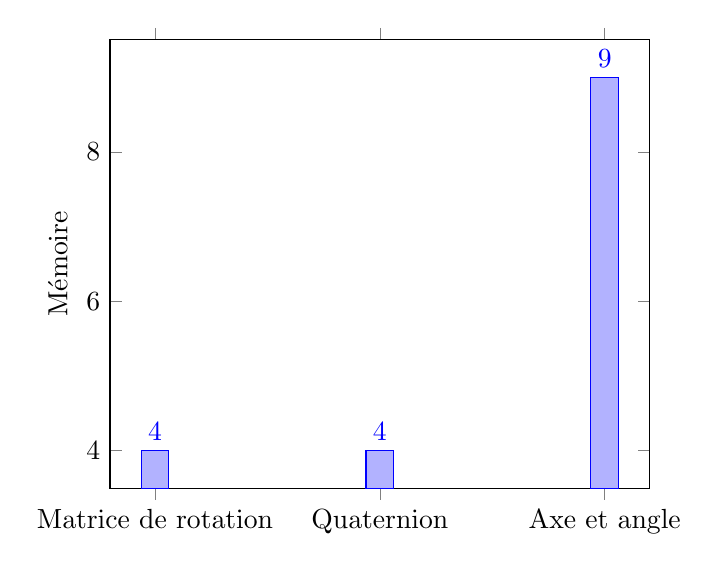
\begin{tikzpicture}
			\begin{axis}[ybar,
			ylabel=Mémoire,
			xtick = data,
			nodes near coords,
			symbolic x coords={Matrice de rotation, Quaternion, Axe et angle}]
			\addplot coordinates {(Matrice de rotation, 4) 
				(Quaternion, 4) (Axe et angle, 9)};
			\end{axis}
		\end{tikzpicture}
		\caption{Utilisation en mémoire}
	\end{subfigure}
	
	\begin{subfigure}[ht]{\linewidth}
		\centering
		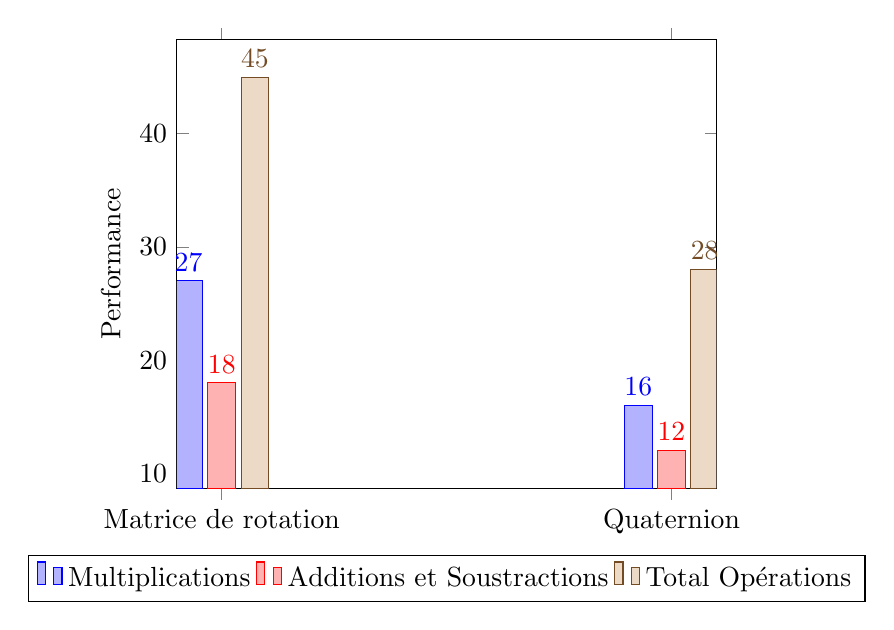
\begin{tikzpicture}
		\begin{axis}[ybar,
		ylabel=Performance,
		xtick = data,
		nodes near coords,
		legend style={at={(0.5,-0.15)},anchor=north,
			legend columns=-1},
		symbolic x coords={Matrice de rotation, Quaternion}]
		\addplot coordinates {(Matrice de rotation, 27) (Quaternion, 16)};
		\addplot coordinates {(Matrice de rotation, 18) (Quaternion, 12)};
		\addplot coordinates {(Matrice de rotation, 45) (Quaternion, 28)};
		\legend{Multiplications, Additions et Soustractions, Total Opérations}
		\end{axis}
		\end{tikzpicture}
		\caption{Performance composition des rotations}
	\end{subfigure}

	\begin{subfigure}[ht]{\linewidth}
		\centering
		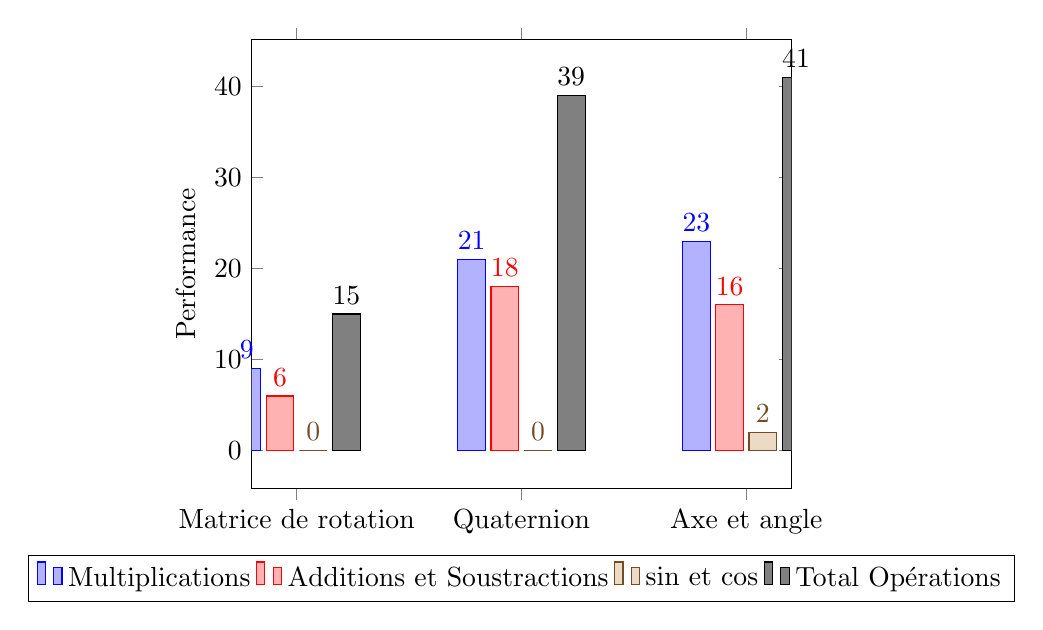
\begin{tikzpicture}
		\begin{axis}[ybar,
		ylabel=Performance,
		xtick = data,
		nodes near coords,
		legend style={at={(0.5,-0.15)},anchor=north,
			legend columns=-1},
		symbolic x coords={Matrice de rotation, Quaternion, Axe et angle}]
		\addplot coordinates {(Matrice de rotation, 9) (Quaternion, 21) (Axe et angle, 23)};
		\addplot coordinates {(Matrice de rotation, 6) (Quaternion, 18) (Axe et angle, 16)};
		\addplot coordinates {(Matrice de rotation, 0) (Quaternion, 0) (Axe et angle, 2)};
		\addplot coordinates {(Matrice de rotation, 15) (Quaternion, 39) (Axe et angle, 41)};
		\legend{Multiplications, Additions et Soustractions, sin et cos, Total Opérations}
		\end{axis}
		\end{tikzpicture}
		\caption{Performance composition des vecteurs}
	\end{subfigure}
\end{figure}

\clearpage